\documentclass[%
	draft,
	paper=a4,%
	abstract=true,%
	]{scrartcl}

\usepackage[utf8]{inputenc}
\usepackage[english]{babel}
\usepackage{graphicx}	
\usepackage{ifpdf}
\usepackage{setspace}
	%\doublespacing
\usepackage{microtype}
\usepackage[colorinlistoftodos]{todonotes}
\usepackage[load-configurations=binary]{siunitx}
	\DeclareSIUnit\Molar{\textsc{m}}
\usepackage{svn-multi}
\usepackage{subfig}
\usepackage{fancyhdr}
\usepackage{tikz}
\usepackage{pgfplots}
\usepackage[numbers,square,sort&compress]{natbib}
\usepackage{scrtime}
\usepackage{lastpage}	
\usepackage[autostyle=true]{csquotes}
%\usepackage{endfloat}
\usepackage{hyperref}

% Subversion Information
\svnidlong
{$HeadURL$}
{$LastChangedDate$}
{$LastChangedRevision$}
{$LastChangedBy$}
\svnid{$Id$} 
 
\pagestyle{fancy}
\fancyfoot{}
\fancyfoot[OR]{\tiny Typeset on \today\ at \thistime\ from \href{\svnkw{HeadURL}}{SVN-Version \svnkw{LastChangedRevision}} | Page \thepage\ of \pageref{LastPage}}
\fancyfoot[EL]{\tiny Page \thepage\ of \pageref{LastPage} | Typeset on \today\ at \thistime\ from \href{\svnkw{HeadURL}}{SVN-Version \svnkw{LastChangedRevision}}}
 
\newcommand{\imsize}{\linewidth}
\newlength\imagewidth		% needed for scalebars
\newlength\imagescale		% ditto

\newcommand{\footremember}[2]{\footnote{#2}\newcounter{#1}\setcounter{#1}{\value{footnote}}}
\newcommand{\footrecall}[1]{\footnotemark[\value{#1}]}

\newcommand{\superscript}[1]{\ensuremath{^{\textrm{#1}}}}
\newcommand{\subscript}[1]{\ensuremath{_{\textrm{#1}}}}

\newcommand{\ie}{i.\,e.\ }
\newcommand{\eg}{e.\,g.\ }

\newcommand{\subfigureautorefname}{\figureautorefname} % make \autoref work with \subfloat
 
\title{How to stereologically characterize individual acini in tomographic datasets of rat lungs\todo{Title: max.\ 160 characters, currently 89.}}
\subtitle{Stereological characterization of individual rat lung acini\todo{Running Head: max.\ 60 char., currently 59.}}

\author{%
	David Haberthür\footremember{ana}{Institute of Anatomy, University of Bern, Switzerland}%
	\and Sébastien Barré\footrecall{ana}%
	\and Stefan Tschanz(?)\footrecall{ana}%
	\and Lilian Salm(?)\footrecall{ana}%
	\and Marco Stampanoni\footremember{psi}{Swiss Light Source, Paul Scherrer Institut, Villigen, Switzerland}\ \footremember{eth}{Institute for Biomedical Engineering, Swiss Federal Institute of Technology and University of Zürich, Switzerland}%
	\and Johannes C. Schittny\footrecall{ana}\ \footremember{contact}{Corresponding Author: Email: \href{mailto:schittny@ana.unibe.ch}{schittny@ana.unibe.ch}, Telephone: +41 31 631 46 35, Fax: +41 31 631 38 07, Address: Institute of Anatomy, University of Bern, Baltzerstrasse 2, CH-3012 Bern}%
	}

\begin{document}
\setcounter{secnumdepth}{-1} % No section numbering, please!
\renewcommand{\subsectionautorefname}{\sectionautorefname} % useful for \autoref
\renewcommand{\subsubsectionautorefname}{\sectionautorefname} % useful for \autoref
\maketitle
\begin{center}
\vfill
Typeset on \today\ at \thistime\ from Rev \svnkw{LastChangedRevision} (\svnday.\svnmonth.\svnyear\ \svnhour:\svnminute)
\vfill
To appear in \emph{\href{http://jap.physiology.org/}{Journal of Applied Physiology}}, \emph{Innovative Techniques}
\vfill
\end{center}
\clearpage

\begin{abstract}
The pulmonary acinus represents the functional unit of the lung. Due to a restricted availability of high resolution imaging methods the knowledge about several biological parameters of  of the acini is limited. Single functional lung units cannot be well characterized from two-dimensional physical sections, due to restrictions imposed by the sectioning method. Our new method builds upon high resolution three dimensional tomographic data obtained by synchrotron radiation based tomographic microscopy. We developed a method to isolate and analyze single acini, to estimate their volume and assess the number of alveoli contained in them. In three-dimensional tomographic datasets we closed the transition between conducting and gas-exchanging airways bronchioles semi-automatically with three-dimensional discs acting as segmentation breakpoints. Our method makes it possible to extract individual acini for volume analysis, something which is not possible on two-dimensional data from single sections of the tissue. The automatic volume analysis of single acini was manually confirmed with stereological assessment. Our proposed method of analyzing single functional units of the mammalian lung is by magnitudes faster than manual stereological analysis of tissue slices and allows to extract biological parameters which can not be extracted from classic single sections. Additionally, the method makes it possible to assess the development of the acini and structural changes in the functional lung units over the postnatal lung development.\todo{One paragraph, no more than 250 words, currently these are 218 words.}
\end{abstract}
	
\section{Keywords}
\begin{itemize}
	\item lung development,
	\item stereology
	\item tomography
	\item acinus
	\item visualization\todo{Three to five words that do not appear in the title or running head}
\end{itemize}
\clearpage
\listoftodos
\clearpage
\todo{Table of contents will be removed, just for overview purposes!}
\tableofcontents

\clearpage
\section{Introduction}
\begin{itemize}
	\item Ausgangspunkt
	\item Was ist bekannt?
	\item \citet{Rodriguez1987} say that (Table 1) the RUL of “Rat” contains 613 acini with a mean volume of \SI{1.98}{\milli\meter\cubed} (\SIrange{0.5}{5}{\milli\meter\cubed}), but specifies no details about the age of the rats.
	\item andere Ausgüsse und Daten erhältlich?
\end{itemize}

Due a restricted availability of high resolution three-dimensional imaging methods the knowledge about the development of the functional unit of the lung is limited. These functional units of the lung parenchyma are the so-called pulmonary acini, which correspond to the gas-exchange volume in the lung which is ventilated by one purely conducting airway~\cite{Rodriguez1987}.

In this manuscript we present a method to isolate and analyze single acini from large high-resolution tomographic datasets. Using datasets obtained with synchrotron radiation based tomographic microscopy with enhanced field of view \cite{Haberthuer2010a}, we extracted individual acini from rat lung samples throughout postnatal lung development. 

Extracting large amounts of single acini from physical sections of lung tissue is extremely time-consuming. \citet{Woodward2005} achieved three-dimensional reconstructions of three adult duck lungs using manual effort to trace serial sections of the tissue. Observing and tracing single acini on microscopy slides for the extraction of their volume is nearly impossible. Tomographic imaging of the lung tissue preserves the three-dimensional structure and makes it trivially easy to extract slices from the imaged tissue.

Since such virtual slices from tomographic datasets do not destroy the three-dimensional structure, we can then carefully isolate and analyze single acini with classic and accepted methods in both two and three dimensions. In addition to three-dimensional volume analysis through segmentation and voxel counting in a visualization software we performed standard stereological analysis \cite{Hsia2010} to compare our results with an accepted ground truth. As stated by \citet{Hsia2010}, Stereology refers to the mathematical methods for analyzing properties of an irregular three-dimensional structure using two-dimensional planar sections obtained by physical or optical imaging techniques.

Extracting single functional lung units from the tomographic datasets enables us to perform such a stereological analysis to obtain a complete description of the functional lung units including alveolar number, surface and volume and compare these values over the course of the postnatal lung development. Such a complete description \todo{We only show volume, should we leave out the rest?} is only possible with tomographic data, since the three-dimensional information in the sample is not destroyed.

\subsection{Lung structure and the functional units of the lung}
The airway structure of the mammalian lung is formed from dichotomous branches~\cite{Weibel1991}, starting from the trachea. The first branching generations lead into the bronchi. With increasing depth into the airway tree, the airway diameter of the airways is reduced, the bronchi are divided into bronchioles, leading to the terminal bronchioles which then mark the end of the pipe-like purely conducting airways. The respiratory bronchioles mark the start of the gas-exchange region in the lung. We start to see changes in the airway wall structure---alveolar outpouchings---and changes in the airway epithelium which both mark the change between purely conducting and gas-exchanging airways (see \autoref{fig:ManholeCoverExplanation}). After this point, the so-called acinar airways and the acinus---the functional unit of the lung---begin. The observation of such changes in the airway wall make it possible to extract single acini from the three-dimensional tomographic datasets, as described later in Materials and Methods.

The lung structure can be assessed using stereology, as shown by \citet{Tschanz2002}. Such an analysis is generally based on two-dimensional physical sections of the sample, thus the extracted information is a two-dimensional description \blockquote[\cite{Tschanz2002}]{of the parenchymal air space geometry and, due to geometric laws, it is not allowed to extrapolate these two-dimensional statements directly to three-dimensional structures}. With stereological methods it is possible to extract global volume information, but it not easily possible to extract such information from a functional subunit of an organ like the acini in the lung, since it cannot easily be assessed which detail on one microscopy slide belongs to which functional unit in the three-dimensional compound. With a three-dimensional segmentation we can extract virtual two-dimensional slices of one isolated functional unit, enabling a thorough stereological characterization of individual acini in the mammalian lung.

\section{Materials and Methods}
\subsection{Rat lung samples}
The results shown in this manuscript have been obtained from lungs from adult Sprague-Dawley rats at day 60 after birth. Animals were deeply anesthetized with a mixture of %
\SI{0.5}{\milli\gram\per\milli\litre} Acetylpromazine, %
\SI{5}{\milli\gram\per\milli\litre} Xylazine and %
\SI{50}{\milli\gram\per\milli\litre} Ketamine in %
\SI{0.9}{\percent} NaCl at \SIrange{1.5}{2.5}{\micro\litre} per \si{\gram} body weight. The lungs of the animals were instilled with \SI{2.5}{\percent} glutaraldehyde in \SI{0.03}{\Molar} potassium-phosphate buffer (pH 7.4) at a constant pressure of \SI{20}{\centi\meter} water column. At this applied pressure, the rat lung reaches its mid-respiratory volume \cite{Schittny1998}. The instillation was performed via tracheotomy after opening the chest cavity and setting a pneumothorax through perforation of the diaphragm. After instillation the lung was removed from the chest cavity and the instillation pressure was maintained during fixation (in the same fixative at \SI{4}{\celsius} for at least \SI{24}{\hour}) in order to prevent a recoiling of the lung \cite{Tschanz2002}.

After fixation, the samples were prepared for tomographic imaging by postfixation with \SI{1}{\percent} osmium acetate and staining with \SI{4}{\percent} uranyl nitrate to increase the x-ray absorption contrast. Using Histoclear (Merck KGaA, Darmstadt, Germany) as an intermedium the samples were then dehydrated in a graded series of ethanol and embedded in paraffin prior to mounting them onto standard scanning electron microscopy sample holders (PLANO GmbH, Wetzlar, Germany) with paraffin~\cite{Tsuda2008}.

The handling of animals before and during the experiments, as well as the experiments themselves, were approved and supervised by the Swiss Agency for the Environment, Forests and Landscape and the Veterinary Service of the Canton of Bern, Switzerland.

\subsection{Tomographic data acquisition}
The tomographic experiments were performed at the \href{http://www.psi.ch/sls/tomcat/}{TOMCAT beamline} at the \href{http://www.psi.ch/sls/}{Swiss Light Source}, \href{http://www.psi.ch/}{Paul Scherrer Institut}, Villigen, Switzerland~\cite{Stampanoni2006a}. The samples were scanned at an x-ray energy of \SI{20.0}{\kilo\electronvolt} corresponding to a wavelength of \(\lambda=\SI{0.62}{\angstrom}\). % \lambda = 1.24e-6 eV/m / 20 keV = 6.197796e-11 m = 0.6197796 Ångström
After penetration through the sample, the x-rays were converted into visible light by---depending on the beamtime---either a \SI{20}{\micro\meter} thick LuAG:Ce (Cerium doped Lutetium Aluminum Garnet, \href{http://www.crytur.cz/}{Crytur Ltd.}, Turnov, Czech Republic) or \SI{18}{\micro\meter} thick YAG:Ce (Cerium doped Yttrium Aluminium Garnet, also by Crytur) scintillator screen. A 10\(\times\) magnifying, diffraction limited microscope optics was used to magnify the scintillator image prior to recording it with a 2048\(\times\)2048 pixel CCD camera (\href{http://www.pco.de/sensitive-cameras/pco2000/}{pco.2000}, \href{http://www.pco.de/}{PCO AG}, Kelheim, Germany) with \SI{14}{\bit} dynamic range. To reduce imaging noise and increase the acquisition speed, we operated the detector in 2\(\times\)2 binning mode. As a result, the pixel size was \SI{1.48}{\micro\meter} and the exposure time was between \SIrange{160}{200}{\milli\second}.

To be able to safely distinguish the alveolar septa which in rats have an mean thickness of \SIrange{5}{10}{\micro\meter} (calculated from data in \citet{Burri1974}) the tomographic images used for analysis of the functional units of the lung need to have a resolution in the order of one to two microns. Since we selectively wanted to extract a large amount of single acini, we not only needed to acquire high resolution tomographic scans, but also acquire dataset with both large volume and high resolution. Usually---with classic microscopy based imaging methods---a large field of view can only be acquired with low magnification and vice-versa. Since our samples were larger than the classic field of view of TOMCAT at the aforementioned optical properties (\(1.52\times1.52\times\SI{1.52}{\milli\meter}\)) we would not have been able to image the desired volume of our samples. To overcome this problem, we recorded tomographic dataset of our samples with the so-called wide field scanning method, described by \citet{Haberthuer2010a}.

Briefly summarized, the wide field scanning process merges several partial tomographic scans perpendicular to the rotation axis of the sample to successively cover the total desired field of view. Additionally, several widefieldscans have been stacked parallel to the rotation axis of the sample in the tomographic setup. The resulting large tomographic datasets had a size of approximately 3000\(\times\)3000\(\times\)3072 pixels with \SI{1.48}{\micro\meter} pixel size, corresponding to a 9-fold increase in recorded volume as compared to a single scan at TOMCAT at the given optical configuration.

\subsection{Visualization and Extraction of Acini}
The tomographic datasets of the sample were three-dimensionally analyzed and visualized using \href{http://mevislab.de}{MeVisLab} (Version 2.1 (2010-07-26 Release)~\cite{Bitter2007}, MeVis Medical Solutions AG and Fraunhofer MEVIS -- Institute for Medical Image Computing, Bremen, Germany). The analysis and visualizations have been performed on a Dell Precision T7500 work station (\SI{24}{\giga\byte} RAM, Intel Xeon CPU X5550 at \SI{2.66}{\giga\hertz}, Windows 7 Professional \SI{64}{\bit}). 

The tomographic datasets obtained at TOMCAT were converted from a stack of TIFF-files to the native GVR format of MeVisLab, a multi-resolution \href{https://secure.wikimedia.org/wikipedia/en/w/index.php?title=Octree&oldid=409131920}{octree}-based image format. This permitted us to easily switch between resolutions in the dataset to interactively perform the visualization and preliminary analysis on a lower resolution prior to the final analysis on full resolution datasets. A graphical user interface was developed using MDL (MeVisLab Definition Language) to facilitate the task of defining regions of interest in the dataset, isolating single functional lung units, extracting them from the tomographic dataset for subsequent verification, visualizing the extracted acini in three-dimensional, analyzing and tabulating their volume.

\subsubsection{Manhole Covers}
We extracted conducting airway segments using a threshold interval based region growing algorithm~\cite{Zucker1976}. To start the extraction, a seed point for the region growing algorithm was manually defined inside the conducting airways on one of the most proximal slices of the dataset (see \autoref{subfig:sample}) as a first step. With this first seed point, one or several connected airway segments was extracted from the lung sample. Such an extracted airways segment was composed of both conducting and gas-exchanging airways. Using segmentation stoppers dubbed manhole covers, we in a second step isolated single acini from each large airway segment until it was cut back to only the conducting airways. These manhole covers are visible as red discs in \autoref{subfig:airway segment} and \subref*{subfig:extracted acini}. The manhole covers were implemented through a \href{http://www.mevis-research.de/cgi-bin/discus/board-auth.cgi?lm=1282233250&file=/839/11760.html}{custom MeVisLab module (\emph{XMarkerClipPlanes})} written by Milo Hindennach, a member of the MeVis Developer team. The locations of the manhole covers were defined based on morphological criteria, \ie changes in the epithelial thickness of the airway wall and appearance of alveolar outpouchings in the airway wall mark the transition from conducting to gas-exchanging airways.

\renewcommand{\imsize}{\linewidth}
\begin{figure}
	\centering
	\pgfmathsetlength{\imagewidth}{\imsize}%
	\pgfmathsetlength{\imagescale}{\imagewidth/953}%
	\def\x{589}% scalebar-x at golden ratio of x=953px
	\def\y{858}% scalebar-y at 90% of height of y=953px
	\begin{tikzpicture}[x=\imagescale,y=-\imagescale]
	\clip (0,0) rectangle (953,953);
		\node[anchor=north west, inner sep=0pt, outer sep=0pt] at (0,0) {\includegraphics[width=\imagewidth]{img/ManholeCoverExplanation/60B_sagittal_slice_415}}; %_scalebar
		% 440px = 2mm > 100px = 455um > 110px = 500um, 22px = 100um
		%\draw[|-|,blue,thick] (868,237) -- (868,677) node [sloped,midway,above,fill=white,semitransparent,text opacity=1] {\SI{2}{\milli\meter} (2000px) TEMPORARY!};
		\draw[|-|,white,thick] (\x,\y) -- (\x+110,\y) node [midway,above] {\SI{500}{\micro\meter}};
		\draw[yellow,dashed,ultra thick] (508,436) circle (20);
		\fill[yellow,nearly transparent] (508,436) circle (20);
		\draw[yellow,dashed,ultra thick] (617,407) circle (20);
		\fill[yellow,nearly transparent] (617,407) circle (20);
		\draw[yellow,dashed,ultra thick] (642,434) circle (20);
		\fill[yellow,nearly transparent] (642,434) circle (20);
		\draw[yellow,dashed,ultra thick] (385,663) circle (20);
		\fill[yellow,nearly transparent] (385,663) circle (20);	
		\draw[yellow,dashed,ultra thick] (347,653) circle (15);
		\fill[yellow,nearly transparent] (347,653) circle (15);
		\draw[yellow,dashed,ultra thick] (245,667) circle (20);
		\fill[yellow,nearly transparent] (245,667) circle (20);	
	\end{tikzpicture}%
	\caption{One sagittal slice of the tomographic dataset of the animal B showing extracted conducting airways in green and several manhole covers in red. The dashed yellow circles highlight some examples of alveolar outpouchings of the airway wall which mark the change from conducting to gas-exchanging regions. Additionally, changes in the epithelial layer of the airway wall, especially changes in thickness and structure also mark this change. Visually assessing these changes made it possible to semiautomatically place manhole covers in the three-dimensional tomographic dataset to isolate single acini from our dataset. Four manhole covers are shown cut right through the middle, two manhole covers are only fractionally cut and thus appear much smaller on this slice.}
	\label{fig:ManholeCoverExplanation}
\end{figure}

Once all acinar openings were defined, we extracted the volume of each isolated acinus (shown as yellow volumes in \autoref{subfig:extracted acini}) in a automatic third step. The manhole covers placed in the steps mentioned before are defined through their diameter and \href{https://secure.wikimedia.org/wikipedia/en/w/index.php?title=Surface_normal&oldid=411684319}{surface normal} in the three-dimensional dataset. To define the seed point for an additional region growing module to extract the acinar volume we simply flipped the direction of the surface normal defining the manhole cover and placed the seed point for the acinar region growing along this vector, slightly behind the manhole cover inside the acinar airspace. The only manual work needed for the final extraction of the volume of each acinus was the iterative selection of the appropriate segmentation threshold and subsequent tabulation of the automatically calculated acinar volume.

\renewcommand{\imsize}{.333\linewidth}%
\pgfmathsetlength{\imagewidth}{\imsize}%
\pgfmathsetlength{\imagescale}{\imagewidth/1008}%
\def\x{50}% scalebar-x at golden ratio of x=1008px
\def\y{916+20}% scalebar-y at 90% of height of y=1018px
\begin{figure}
	\centering
	\subfloat[Sample]{%
		\begin{tikzpicture}[x=\imagescale,y=-\imagescale]
			\node[anchor=north west, inner sep=0pt, outer sep=0pt] at (0,0) {\includegraphics[width=\imagewidth]{img/ManholeCover/R108C60B_2010c_Acinus_Sample}};
			% 774px = 4.363mm > 100px = 564um > 89px = 500um, 18px = 100um
			%\draw[|-|,blue,thick] (775,990) -- (33,771) node [sloped,midway,above,fill=white,semitransparent,text opacity=1] {\SI{4.363}{\milli\meter} (2948px) TEMPORARY!};
			\draw[|-|, thick] (\x,\y) -- (\x+89,\y) node [right] {\SI{500}{\micro\meter}};
		\end{tikzpicture}%
		\label{subfig:sample}%
		}%
	\subfloat[Extracted conducting airways with manhole covers shown overlaid over Sample.]{%
		\begin{tikzpicture}[x=\imagescale,y=-\imagescale]
			\node[anchor=north west, inner sep=0pt, outer sep=0pt] at (0,0) {\includegraphics[width=\imagewidth]{img/ManholeCover/R108C60B_2010c_Acinus_Airspace_Overlay}};
			\draw[|-|, thick] (\x,\y) -- (\x+89,\y) node [right] {\SI{500}{\micro\meter}};
		\end{tikzpicture}%
		\label{subfig:airway segment}%
		}%
	\subfloat[Extracted acini.]{%
		\begin{tikzpicture}[x=\imagescale,y=-\imagescale]
			\node[anchor=north west, inner sep=0pt, outer sep=0pt] at (0,0) {\includegraphics[width=\imagewidth]{img/ManholeCover/R108C60B_2010c_Acinus_OverlayNonTransparent}};
			% 774px = 4.363mm > 100px = 564um > 89px = 500um, 18px = 100um
			\draw[|-|, thick] (\x,\y) -- (\x+89,\y) node [right] {\SI{500}{\micro\meter}};
		\end{tikzpicture}%
		\label{subfig:extracted acini}%
		}
	\caption{Visualization of the work flow for the extraction of the acinar volumes on a rat lung sample extracted at day 60: %
		\subref{subfig:sample}: three-dimensional visualization of a sample. To increase the field of view nine-fold compared to a classic scan at TOMCAT we stacked three wide field scans on top of each other. The borders between the three stacked scans are faintly visible as darker lines, but are only visible in this three-dimensional visualization and did not influence the three-dimensional reconstruction. %
		\subref{subfig:airway segment} Extracted airway segment (green) superimposed on the sample. Using a threshold based region growing algorithm, we extracted conducting airways inside the sample. The red discs shown are the so-called manhole covers, which were semiautomatically placed and used as segmentation stoppers for the region growing. %
		\subref{subfig:extracted acini} Extracted acini (yellow). Multiple extracted acini are shown superimposed over the sample in three-dimensional. For each such acinus we recorded the volume.%
		}
	\label{fig:workflow}
\end{figure}

The volume of the single acini was calculated by multiplying the amount of segmented voxels with the voxel volume, tabulated in Excel-Files and prepared for analysis. Each segmented acinus was exported as single \href{https://secure.wikimedia.org/wikipedia/en/w/index.php?title=Digital_Imaging_and_Communications_in_Medicine&oldid=415023605}{DICOM} files for further processing as described below.

\subsection{Stereological Analysis and comparison of acinar volumes obtained with different methods}
The volume of the single acini was automatically calculated from the amount of segmented voxels multiplied by their size. To check these volumes against a gold standard method, we stereologically estimated the volume of single exemplary acini. To guarantee accurate and unbiased results, we standardized each step of tissue fixation, processing sampling and analysis and performed the stereological assessment according to official guidelines, as specified by \citet{Hsia2010}.

For this analysis, we prepared datasets in which we combined each segmented acinus with the corresponding region of interest from the original tomographic dataset, as seen in the background of \autoref{fig:STEPanizer} and exported these regions of interest as DICOM files. With a MATLAB script we padded the volumes to a square format, systematically randomly sampled and exported as JPG sequences for further stereological analysis.

Using a web based tool developed at our institute, the so-called STEPanizer \cite[available free of charge at \url{http://stepanizer.com}]{Tschanz2011} we analyzed the volume and surface of the extracted acini. With the STEPanizer we counted intersections of the acinar surface with geometric line probes for the surface and performed point counting to assess the volume of the extracted acini. \autoref{fig:STEPanizer} shows one such exported slice while being analyzed using the STEPanizer. Counting points (green three-quarter circles) and intersections (red \href{https://encrypted.google.com/search?q=i-beam&tbm=isch}{I-beam}-shaped lines) are overlaid to count both the points inside the acinar volume and intersections with the acinar surface. The measurements are exported to \href{https://secure.wikimedia.org/wikipedia/en/w/index.php?title=Comma-separated_values&oldid=441921632}{csv}-delimited tables for further analysis. This process made it possible to relate the automatically calculated volumes from MeVisLab to an accepted and proven stereological method.

\renewcommand{\imsize}{\linewidth}%
\begin{figure}
	\centering
	\includegraphics[width=\imsize]{img/STEPanizer_2010_R108C60B_acinus01_Slice75}
	\caption{STEPanizer counting window. The segmented acinus is visible in light gray, the manhole cover is show as darker gray rectangle (another manhole cover from an adjacent acinus is partially visible at the top of the image). Both structures are overlaid and merged with the original tomographic data in the background. Line and point probes (red lines and green circles) are overlaid over the image for counting. To correctly count all structures in the image, the original non-square datasets have been padded to a square, resulting in the white rectangle at the lower border of the image. Scalebar: \SI{100}{\micro\meter}.}
	\label{fig:STEPanizer}
\end{figure}

\section{Results}
\todo{Absolute Volumina müssen rein}
Was wurde gemacht?
\begin{itemize}
	\item Volume
	\item Surface
	\begin{itemize}
		\item Coast of Wales-Problem
		\item Triangulation der Oberfläche -> deshalb nur von Hand ausgezählt (“Results not shown”?)
	\end{itemize}
	\item Number of Acini
\end{itemize}

\subsection{Comparison of Volumes from MeVisLab with STEPanizer}
For four animals obtained at postnatal day 60 we isolated 165 individual acini. For 48 of these acini \todo{Latest numbers from ‘STEPanizerReaderAndPlotter.m’?} we compared the automatically detected volume of MeVisLab with manual stereological counting. Normalizing the volumes to the volume obtained with MeVisLab made it possible to assess differences between the two methods. The results are shown in \autoref{fig:VolumeMeVisVsSTEPanizer} and explained later on in the Discussion section.

\begin{figure}
	\centering
	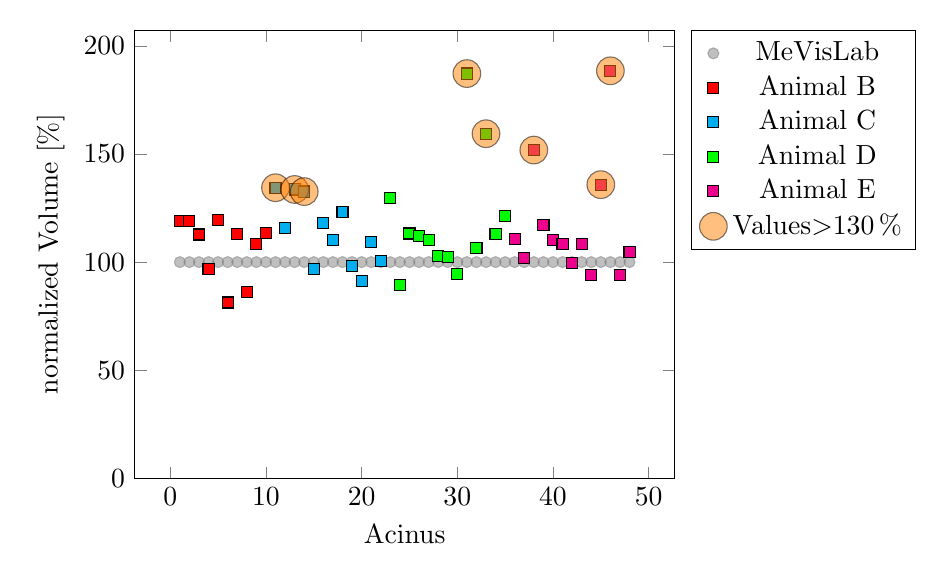
\begin{tikzpicture}
		\begin{axis}[%
			only marks,
			legend pos=outer north east,
			ymin=0,
			xlabel=Acinus,
			ylabel={normalized Volume [\si{\percent}]}
			]
			\addplot [semitransparent,gray,mark=*]
				coordinates{
					(1,100) (2,100) (3,100) (4,100) (5,100) (6,100) (7,100) (8,100) (9,100) (10,100) (11,100) (12,100) (13,100) (14,100) (15,100) (16,100) (17,100) (18,100) (19,100) (20,100) (21,100) (22,100) (23,100) (24,100) (25,100) (26,100) (27,100) (28,100) (29,100) (30,100) (31,100) (32,100) (33,100) (34,100) (35,100) (36,100) (37,100) (38,100) (39,100) (40,100) (41,100) (42,100) (43,100) (44,100) (45,100) (46,100) (47,100) (48,100)
				};
				\label{plot:mevis}
			\addplot [fill=red, draw=black, mark=square*]
				coordinates{
					(1,118.844) (2,118.888) (3,112.751) (4,96.6436) (5,119.518) (6,81.3158) (7,112.81) (8,86.1239) (9,108.54) (10,113.4)
					};
				\label{plot:animalb}
			\addplot [fill=cyan, draw=black, mark=square*]
				coordinates{
					(11,134.386)
					(12,115.871)
					(13,133.579) (14,132.599)
					(15,96.8582) (16,117.926) (17,110.275) (18,123.272) (19,98.1566) (20,91.4073) (21,109.274) (22,100.527)
					};
			\addplot [fill=green, draw=black, mark=square*]
				coordinates{
					(23,129.824) (24,89.3898) (25,113.225) (26,112.215) (27,110.095) (28,102.662) (29,102.433) (30,94.6387)
					(31,187.167)
					(32,106.537)
					(33,159.367)
					(34,113.17) (35,121.325)
					};		
			\addplot [fill=magenta, draw=black, mark=square*]
				coordinates{
					 (36,110.653) (37,101.875)
					 (38,151.8)
					 (39,117.306) (40,110.189) (41,108.314) (42,99.5121) (43,108.438) (44,94.2065)
					 (45,135.812) (46,188.439)
					 (47,94.0823) (48,104.747)
				};
				\label{plot:animale}
			\addplot[fill=orange, draw=black, mark=*,mark size=5,semitransparent]
				coordinates{
					(11,134.3863)
					(13,133.5789)
					(14,132.599)
					(31,187.1668)
					(33,159.3669)
					(38,151.7996)
					(45,135.8118)
					(46,188.439)
				};
				\label{plot:removed}
			\legend{MeVisLab,Animal B,Animal C,Animal D,Animal E,Values\(>\)\SI{130}{\percent}}
		\end{axis}
	\end{tikzpicture}
	\caption{Volumes of different acini estimated with different Methods. The volumes have been normalized to the volume obtained with MeVisLab (\ref{plot:mevis}). The average volume of a single acinus is \SI{10}{\percent} larger when assessed with the STEPanizer (\ref{plot:animalb}--\ref{plot:animale}) as compared to MeVisLab (\SI{106.931}{\percent} vs.\ \SI{100}{\percent}). %
		See the Discussion for an explanation of the yellow data points (\ref{plot:removed}) which were removed from analysis since they showed values larger than \SI{130}{\percent}.}%
	\label{fig:VolumeMeVisVsSTEPanizer}%
\end{figure}

As expected, both methods show slightly different results. The automatic method based on a threshold interval region growing segmentation of the three-dimensional data in MeVisLab showed slightly lower volumes for the acini than a manual stereological analysis did. \autoref{fig:VolumeMeVisVsSTEPanizer} shows a plot of the acinar volumes normalized to the automatic method. Since the automatic calculation of the acinar volume with MeVisLab simply adds up all segmented voxels, an imprecise segmentation leads to an underestimation of the acinar volume. \autoref{fig:MeVisSegmentation} shows exemplary slices for acini with large differences in volume between the two methods. Due to inevitable segmentation inaccuracies (dark spots inside the segmented acinus in \autoref{subfig:60d_acinus32} we underestimated the volumes with the automatic method compared to the manual, stereological method, where we visually discard such inaccuracies.

In some extracted acini we have seen differences in gray values in the z-direction of the stack. Since the region growing segmentation method uses the same threshold throughout the region of interest, sometimes single slices were heavily under-estimated in terms of included voxels, one such example is shown in \autoref{subfig:60e_acinus38}. Since these automatically extracted regions were merely used as a optic guidance for the manual, stereological method it is obvious that the manual method shows slightly larger volumes (\SI{6.931}{\percent} larger\todo{Correct? Use ‘STEPanizerReaderAndPlotter.m’ for latest value!}) than the automatic method.

\section{Discussion}
\todo{Kurze Wiederholung der Resultate}
Applying our novel method dubbed manhole cover segmentation to tomographic datasets of 4 animals we extracted nearly 200 acini to analyze their volume. With this semiautomatic method we are able to isolate and analyze individual acini in both a two- and three-dimensional way using widely accepted methods like voxel counting and Stereology. We have shown that we can automatically calculate the volume of single acini in mammalian lungs from three-dimensional tomographic data and match the accuracy of a manual method while performing the analysis orders of magnitude faster. Only with this novel combination of methods it is possible to accurately assess the volume of single acini in three-dimensional tomographic data.

Our proposed method opens up the possibility to fully analyze biologically interesting parameters of the acini in the lung; the volume of the acini can be extracted automatically, parameters like surface as well as number of contained alveoli and septal length per acinus can be extracted with simple stereological counting, but require manual labour. These parameters can be obtained for single isolated acini, something which is not easily possible using stereological methods on classic tissue sections.

\subsection[Comparison of MeVisLab with STEPanizer]{Comparison of automatic stereology with MeVisLab and manual stereology with the STEPanizer}
Manually assessing the volume of the single acini using the STEPanizer took several working days for the few acini shown in \autoref{fig:VolumeMeVisVsSTEPanizer}. As soon as the manhole covers are defined in the sample, the automatic volume calculation with MeVisLab can be performed in less than a minute per acinus. Even though we slightly underestimate the volume of the single acini with the automatic method, we simply could not manually assess the volume for each one of the nearly 200 acini of postnatal day 60\todo{Do we never mention the 1000 acini I totally assessed?}. We have shown that our automatic method can be validated with a proven and accepted gold standard method.

Additionally, in the final study we will not look at the absolute volume, but only at the volume fractions or increase of volume, so this difference in absolute volume can be neglected for our purposes.

\todo{Fehler ist im Bereich des Messfehlers, Underestimation liegt an der Mess-Methode}
\todo{Vorhandene Daten diskutieren. Silikonausgüsse von \citet{Rodrigues1987}, etc.\ diskutieren.}
\todo{Wir können strukturelle Änderungen im Acinus untersuchen! Entwicklung, Krankheit und Knock-Out-Tiere mit strukturellen Veränderungen können angeschaut werden!}

\renewcommand{\imsize}{0.56\linewidth}%
\begin{figure}
	\centering
	\hfill%
	\subfloat[60D, Acinus 32, Slice 45, Vol.\ \SI{159}{\percent}]{%
		\includegraphics[height=\imsize]{img/Acini/2009f/mrg/R108C60Dt-mrg/acinus32/voxelsize1.48-every6slice/R108C60Dt-mrg-acinus32_45.png}% jpg is unedited!
		\label{subfig:60d_acinus32}%
	}%
	\hfill%
	\subfloat[60E, Acinus 38, Slice 29, Vol.\ \SI{188}{\percent}]{%
		\includegraphics[height=\imsize]{img/Acini/2009f/mrg/R108C60Et-mrg/acinus38/voxelsize1.48-every6slice/R108C60Et-mrg-acinus38_29.png}% jpg is unedited!
		\label{subfig:60e_acinus38}%		
	}%
	\hfill%
	\caption{Illustrative slices of two acini that show large differences in volume between MeVisLab and STEPanizer. The inaccurate segmentation is the reason we obtained larger volumes with the STEPanizer than with MeVisLab. The image in panel \subref{subfig:60d_acinus32} shows minor segmentation errors through noise in the paraffin (dark spots inside grey region). The image in panel \subref{subfig:60e_acinus38} shows large segmentation errors. Such large errors arise through brightness changes in the dataset which render the global threshold unusable for certain slices. Scalebar: \SI{100}{\micro\meter}.}
	\label{fig:MeVisSegmentation}
\end{figure}

\subsection{Conclusions}
The hereby presented manhole cover method is well suited to semi-automatically isolate the functional lung units from three-dimensional datasets. The presented workflow permits a fully automated analysis of the volume of the functional lung units and enables the study of large amounts of acini in relatively short time.\todo{Shall we write something about the 1000 extracted acini for days \numrange{4}{60}?}

We validated our automatic method with a proven and accepted method, the so-called Stereology. We have shown that---even though there are slight differences between the two methods---the achieved results are comparable. Since our proposed method for assessing the volumes of isolated individual acini is by magnitudes faster than manual stereological counting, we believe the presented method is the easiest and fastest way to assess the volume of single acini in the mammalian lungs.

\clearpage
\section{Acknowledgments}
We thank Federica Marone, Christoph Hintermüller and Bernd Pinzer for the great support at the TOMCAT Beamline. Milo Hindennach from Fraunhofer MEVIS provided the \href{http://www.mevis-research.de/cgi-bin/discus/board-auth.cgi?lm=1282233250&file=/839/11760.html}{Manhole cover module in MeVisLab}. We thank Mohammed Ouanella and Eveline Yao for expert technical assistance and embedding of the samples.

This work has been funded by the grants 3100A0-109874 and 310030-125397 of the Swiss National Science Foundation.

\clearpage
\singlespacing
\bibliographystyle{plainnat}
\bibliography{../references}

\end{document}